\documentclass[11pt,a4paper]{article}
\usepackage[T1]{fontenc}
\usepackage[utf8]{inputenc}
\usepackage[margin=25mm]{geometry}
\usepackage{amsmath,amssymb,booktabs,graphicx,microtype}
\usepackage{hyperref}
\usepackage[backend=biber,style=numeric,sorting=none,maxbibnames=10]{biblatex}
\addbibresource{references.bib}
\hypersetup{colorlinks=true,urlcolor=blue,citecolor=blue,linkcolor=blue}
\title{Finite-Calibration Bounds for Correlated-Noise Decoders in a 3-Qubit Repetition Code}
\author{QEC-R01 research draft\\\small Author names and affiliations to be confirmed before submission}
\date{25 October 2026\\\small Working preprint---not submitted or peer reviewed}
\begin{document}
\maketitle
\begin{abstract}
We examine finite-shot calibration of a maximum-a-posteriori (MAP) decoder for the three-qubit bit-flip repetition code under independent Pauli-$X$ noise and an additional correlated two-qubit $X$ event. Known-state calibration samples estimate the pair-event probability; decoder choices are evaluated by exact enumeration of eight $X$-error masks. At independent flip probability $p=0.02$, paired-event probability $b=0.04$, and 2,000 calibration replicates per sample size, $N=1000$ shots select the oracle decoder branch in 1,995/2,000 replicates (99.75\%; Wilson 95\% interval 99.416--99.893\%). The mean conditional exact logical $X$-failure rate is 0.02004896, versus 0.039584 for minimum-weight decoding, an improvement of 1.953504 percentage points. We derive the exact binomial selection probability and a conservative finite-sample bound. This is a one-round, $X$-only code-capacity model, not a circuit-level or quantum-device demonstration; a separate QuTiP amplitude-damping experiment was blocked by the runtime environment.
\end{abstract}

\section{Introduction}
Quantum error correction (QEC) stores information redundantly and relies on syndromes to infer recovery operations \cite{gottesman1997,ibmrepetition}. The decoder's choice among errors consistent with a syndrome depends on the prior distribution of faults. Real noise correlations can therefore change the preferred recovery. Optimization of decoder priors has already been investigated experimentally for repetition and surface codes \cite{sivak2024}. IBM Quantum researchers have compared matching and maximum-likelihood decoders in multi-round experiments \cite{sundaresan2023}; IBM devices also support more sophisticated topological-code demonstrations \cite{hetenyi2024}. No claim of priority for correlation-aware decoding is made here.

Our deliberately narrow question is how finite calibration of one paired-$X$ noise parameter affects decoder selection and conditional logical error in an exactly enumerable three-data-qubit model. This construction protects against isolated $X$ errors; it does not correct arbitrary single-qubit Pauli errors.

\section{Methods}
\subsection{Three-qubit code and correlated-\texorpdfstring{$X$}{X} noise}
The logical computational states are $|0_L\rangle=|000\rangle$ and $|1_L\rangle=|111\rangle$, with $X$-syndrome generators $Z_0Z_1$ and $Z_1Z_2$. For a mask $e=(e_0,e_1,e_2)$, the ideal syndrome is
\begin{equation}
 s(e)=(e_0\oplus e_1,\;e_1\oplus e_2).
\end{equation}
Draw independent $Z_i\sim\mathrm{Bernoulli}(p)$ and $B\sim\mathrm{Bernoulli}(b)$, and form
\begin{equation}
 E=(Z_0,Z_1,Z_2)\oplus(B,B,0),\qquad p=0.02.
\end{equation}
The additional paired fault can cancel independent flips under XOR. For $u=(1,1,0)$ and Hamming weight $w$, the probability of mask $e$ is
\begin{equation}
 P_{p,b}(e)=(1-b)p^{w(e)}(1-p)^{3-w(e)}+b\,p^{w(e\oplus u)}(1-p)^{3-w(e\oplus u)}.
 \label{eq:noise}
\end{equation}
The two masks for each syndrome differ by $(1,1,1)$. The exact conditional logical $X$-failure rate for decoder $D$ is
\begin{equation}
 L(D;p,b)=\sum_{e\in\{0,1\}^3}P_{p,b}(e)\,\mathbf{1}\{e\oplus D[s(e)]=(1,1,1)\}.
 \label{eq:ler}
\end{equation}

\subsection{MAP decoding and finite calibration}
The minimum-weight baseline chooses the lowest-weight mask consistent with a syndrome. A correlated MAP decoder instead chooses
\begin{equation}
 D_{\rm MAP}(s;\hat b)=\mathop{\rm arg\,max}_{e:s(e)=s}P_{p,\hat b}(e),
\end{equation}
with minimum-weight tie breaking. For the ambiguous syndrome containing $u=(1,1,0)$, the fitted MAP decoder selects the pair-event mask precisely when
\begin{equation}
 \hat b>b_*:=p(1-p)=0.0196.
 \label{eq:threshold}
\end{equation}
This value is a \emph{decision threshold} of the toy model, not an accuracy threshold for fault-tolerant QEC.

Each calibration experiment uses freshly prepared $|000\rangle$ reference states, noisy evolution under Eq.~\eqref{eq:noise}, and computational-basis measurement of physical bit 0. Its marginal excitation probability is $q_0=p+(1-2p)b$. Given $K$ ones in $N>0$ observations,
\begin{equation}
 K\sim\mathrm{Binomial}(N,q_0),\qquad \hat b=\operatorname{clip}_{[0,0.08]}\left(\frac{K/N-p}{1-2p}\right).
 \label{eq:estimator}
\end{equation}
For $N=0$ we always select the baseline. Calibration data are never reused as evaluation labels: for each fitted decoder, Eq.~\eqref{eq:ler} gives the \emph{exact} eight-mask logical failure probability under the fixed true parameters.

\subsection{Finite-calibration probabilities and bounds}
For $b=0.04$, $q_0=0.0584$ and $q_*=p+(1-2p)b_*=0.038816$. The correct oracle branch is chosen if $K\ge\lfloor Nq_*\rfloor+1$. Thus, conditional on the model,
\begin{equation}
 \pi_N=\Pr\{K\ge\lfloor Nq_*\rfloor+1\}
 =\sum_{k=\lfloor Nq_*\rfloor+1}^{N}\binom Nk q_0^k(1-q_0)^{N-k}.
 \label{eq:binomial}
\end{equation}
Since $q_*<q_0$, the Bernoulli Chernoff inequality yields the conservative bound
\begin{equation}
 1-\pi_N=\Pr\{K/N\le q_*\}\le\exp[-N D_{\rm KL}(q_*\Vert q_0)],
 \label{eq:bound}
\end{equation}
where $D_{\rm KL}(a\Vert c)=a\ln(a/c)+(1-a)\ln[(1-a)/(1-c)]$. At $N=1000$, Eq.~\eqref{eq:bound} is approximately 0.01963 for wrong-branch selection, while Eq.~\eqref{eq:binomial} gives approximately 0.002322. These are conditional probability statements, not universal QEC bounds.

\subsection{Executed protocol and reproducibility}
For each $N\in\{0,50,200,1000,5000\}$, 2,000 independent calibration datasets were generated with Python's seeded pseudorandom generator (seed $20261025+N$), with $p=0.02$, $b=0.04$ fixed. Wilson 95\% intervals on the branch frequency quantify simulation-replicate uncertainty, not hardware uncertainty. The \href{https://github.com/Vahiff/qec-r01-public}{public QEC-R01 repository} archives the source files and calibration JSON. From the project root:
\begin{quote}\ttfamily\small
python -m unittest discover -s tests -v\\
python src/calibration.py --replicates 2000\\
--seed 20261025 --output results/calibration.json
\end{quote}
\section{Results}
Table~\ref{tab:calibration} reports the archived Phase-2 primary condition. Minimum-weight decoding gives the exact logical $X$-failure rate $0.039584$, and oracle MAP with known $b$ gives $0.020000$. With $N=1000$, the oracle branch was selected $1995/2000$ times ($0.9975$), with a Wilson 95\% interval $[0.99416,0.99893]$. Averaging each selected decoder's \emph{exact conditional} logical failure rate over calibration replicates yields $0.02004896$, an improvement of 1.953504 percentage points over minimum-weight decoding.
\begin{table}[htbp]
\centering
\caption{Fixed true $b=0.04$; 2,000 calibration replicates per $N$. Logical error is the replicate average of exact eight-mask failure probabilities, not a device measurement. Gain is in percentage points.}
\label{tab:calibration}
\small
\begin{tabular}{@{}rrrrr@{}}
\toprule
$N$ & Oracle branch & Fraction (\%) & Logical $X$ error (\%) & Gain (pp)\\
\midrule
0    & 0/2000    & 0.00   & 3.958400 & 0.000000\\
50   & 1596/2000 & 79.80  & 2.395597 & 1.562803\\
200  & 1799/2000 & 89.95  & 2.196819 & 1.761581\\
1000 & 1995/2000 & 99.75  & 2.004896 & 1.953504\\
5000 & 2000/2000 & 100.00 & 2.000000 & 1.958400\\
\bottomrule
\end{tabular}
\end{table}
The exact finite-sample formula of Eq.~\eqref{eq:binomial} predicts $\pi_{1000}\simeq0.997678$, consistent with the observed $0.9975$. The $N=0$ point is a deterministic baseline; it should not be interpreted as a binomial calibration estimate. Figures~\ref{fig:selection} and~\ref{fig:logical} show the original project plots, copied from \texttt{results/figures/} into this self-contained paper bundle.

\begin{figure}[htbp]
\centering
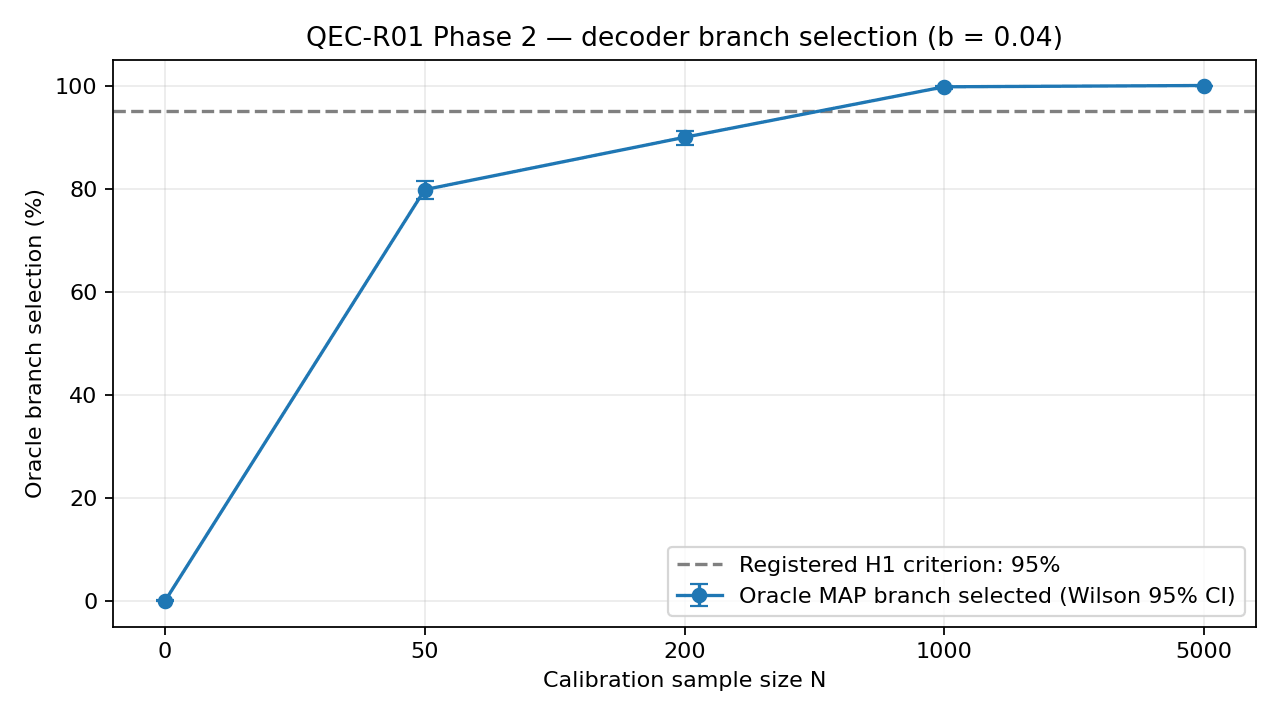
\includegraphics[width=0.94\linewidth]{figures/calibration_branch_selection.png}
\caption{Observed fraction selecting the oracle MAP branch, with Wilson 95\% intervals over 2,000 calibration replicates. The horizontal 95\% line is the predeclared H1 performance criterion, not a statistical significance cutoff.}
\label{fig:selection}
\end{figure}
\begin{figure}[htbp]
\centering
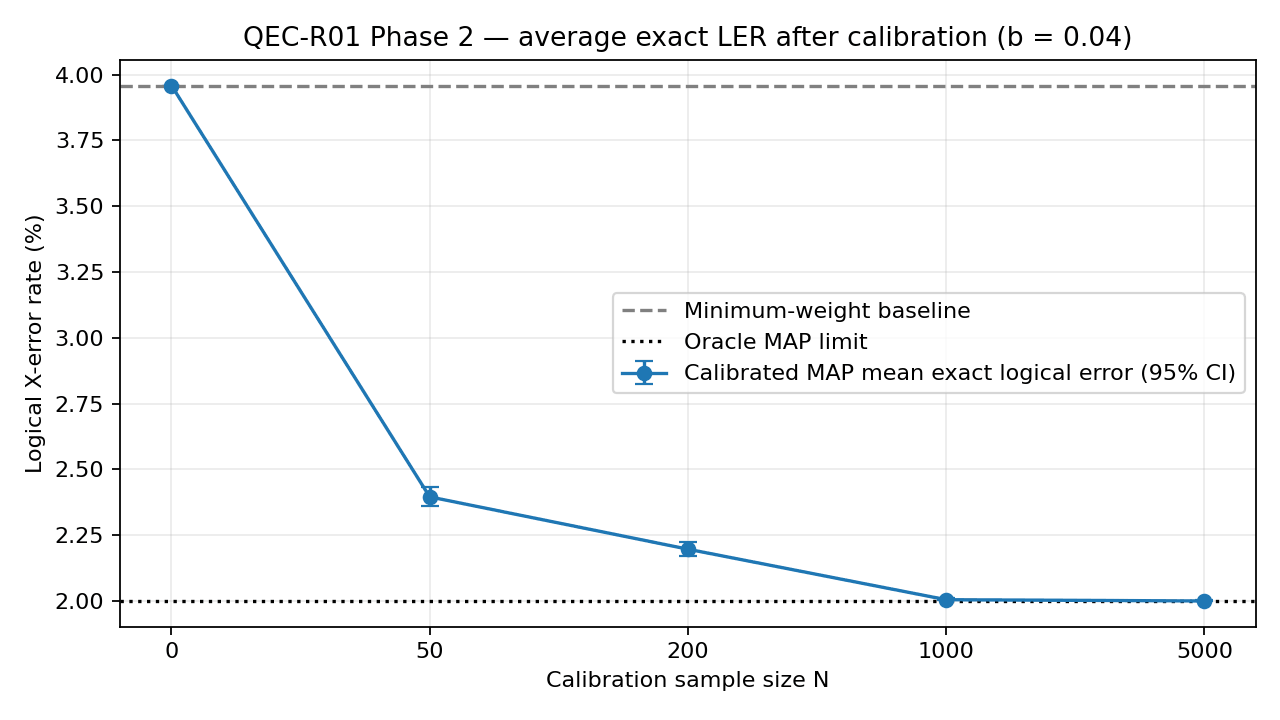
\includegraphics[width=0.94\linewidth]{figures/calibration_logical_error.png}
\caption{Mean of exact conditional logical $X$-failure rates for the decoder chosen by each calibration. Baseline/oracle horizontal references follow exact eight-mask enumeration. Interval bars propagate Wilson bounds on oracle-branch selection, not separate evaluation Monte Carlo.}
\label{fig:logical}
\end{figure}

\section{Limitations and Discussion}
The model is a single-round, \textbf{code-capacity $X$-only} description with perfect syndrome readout: no gate faults, measurement errors, leakage, drift, $Y/Z$ noise, or experimental data. The one-bit estimator assumes exactly known $p$ and access to independently prepared reference states, and estimates one artificial pair-event parameter clipped to $[0,0.08]$. Only the primary true $b=0.04$ case of the registered noise-strength grid was executed; the other points and independent evaluation-shot Monte Carlo for fitted decoders remain \textbf{NOT RUN}. Confidence intervals are conditional on the specified pseudorandom calibration experiment. A complete novelty review and independent experimental validation remain \textbf{NOT VERIFIED}.

A separate QuTiP 5.3.1 density-matrix simulation with amplitude damping was implemented as \texttt{src/qutip\_sim.py}, but \textbf{was not run}: QuTiP was absent and package installation failed on DNS name resolution. This paper does not report fake QuTiP-generated numbers or graphs; an analytical relaxation reference in the project is clearly marked \texttt{NOT\_QUTIP}.

A three-physical-qubit code cannot encode an unknown logical qubit while perfectly correcting arbitrary single-site $X$, $Y$, and $Z$ faults. Such a code would require distance $d\ge3$, but the quantum Singleton bound $n-k\ge2(d-1)$ gives $2\ge4$ for hypothetical $[[3,1,3]]$, a contradiction \cite{gottesman1997}. The smallest general one-error-correcting code uses five physical qubits \cite{laflamme1996}; the nine-qubit Shor code should not be confused with the three-qubit repetition construction.

The contribution of this note is a limited but reproducible calibration case study with an exact binomial selection formula and a conservative finite-sample tail bound. The measured calibration-branch frequencies are neither a novel QEC decoder nor a quantum-device benchmark. Any external submission should follow author/affiliation confirmation, fuller literature review, independent code checks, and a clear statement of the incomplete noise-grid study.

\section*{Code and Data Availability}
The \href{https://github.com/Vahiff/qec-r01-public}{public QEC-R01 repository} contains code and numerical records. Manuscript sources and the copied plots are in \texttt{paper/}. The current draft omits unverified author identities and affiliations. No arXiv submission has occurred.

\printbibliography[heading=bibintoc,title={References}]
\end{document}
